
\section{طرح کوئری }
DBMS
یک کد SQL را به یک طرح کوئری تبدیل می‌کند. عملگرهای طرح کوئری به صورت یک درخت چیده می‌شوند. داده‌ها از برگ‌های این درخت به سمت ریشه این درخت جرکت می‌کنند. خروجی ریشه در درخت نتیجه کوئری است. معمولاً عملگرها باینری (1-2 فرزند دارند) هستند. یک درخت پرس و جو می‌تواند به چندین روش تشکیل و اجرا شود.

\section{مدل‌های پردازشی}
مدل پردازش DBMS مشخص می‌کند که سیستم چگونه یک برنامه پرس و جو را اجرا کند. این مدل چیزهایی مانند جهت ارزیابی کوئری و نوع داده‌هایی که بین عملگرها در طول مسیر منتقل می‌شود را تعیین می‌کند. مدل‌های پردازش مختلفی وجود دارند که برای بارهای کاری مختلف دارای مزایا و معایب متفاوتی نسبت به هم هستند.

این مدل‌ها همچنین می‌توانند به گونه‌ای پیاده‌سازی شوند که عملگرها را از بالا به پایین یا از پایین به بالا فراخوانی کنند. اگرچه رویکرد بالا به پایین بسیار رایج‌تر است، اما رویکرد پایین به بالا می‌تواند کنترل بهتری بر حافظه‌های نهان (کش‌) و ثبات‌ها در خطوط لوله پردازنده فراهم کند.

سه مدل اجرایی که در ادامه مورد بررسی قرار می‌گیرند عبارتند از:


\begin{itemize}
	\item مدل Iterator
	\item مدل Materialization
	\item مدل Vectorized-Batch
\end{itemize}

\subsection{مدل Iterator}

این مدل که به عنوان مدل Pipeline شناخته می‌شود، رایج‌ترین مدل پردازش است و تقریباً توسط هر DBMS مبتنی بر ردیف استفاده می‌شود.

مدل Iterator با پیاده‌سازی یک تابع Next برای هر عملگر در پایگاه داده کار می‌کند. هر Node در برنامه پرس‌وجو تا زمانی که به برگ می‌رسد، Next را بر روی فرزندان خود فراخوانی می‌کند که شروع به ارسال ردیف‌ها به گره‌های پدر خود برای پردازش می‌کنند. 
سپس هر ردیف تا حد امکان به سمت بالا در برنامه پردازش می‌شود قبل از اینکه ردیف بعدی بازیابی شود. این در سیستم‌های مبتنی بر دیسک مفید است زیرا به ما اجازه می‌دهد هر ردیف را در حافظه به طور کامل استفاده کنیم قبل از این که به ردیف یا صفحه بعدی دسترسی پیدا کند. 

\pagebreak

عملگرهای برنامه پرس‌وجو در یک مدل Iterator بسیار قابل ترکیب و آسان برای استدلال هستند زیرا هر عملگر می‌تواند به طور مستقل از عملگرهای پدر یا پسر خود در درخت برنامه پرس‌وجو پیاده‌سازی شود، به شرطی که یک تابع Next را به صورت زیر پیاده‌سازی کند:

\begin{enumerate}
	\item 
	در هر فراخوانی Next ، عملگر یا یک ردیف را برگرداند یا یک پوینتر null .
	\item 
	عملگر باید یک حلقه را پیاده‌سازی کند که Next را بر روی فرزندان خود Call می‌کند تا ردیف‌های آنها را بازیابی کند و سپس آنها را پردازش کند.
	
	به این ترتیب، فراخوانی Next بر روی یک والد، Next را بر روی فرزندان خود فراخوانی می‌کند و در پاسخ گره فرزند ردیف بعدی را که والد باید پردازش کند، برمی‌گرداند.
	
\end{enumerate}


مدل Iterator اجازه می‌دهد تا جایی که ممکن است، DBMS یک ردیف را از طریق عملگرهای مختلف پردازش کند قبل از اینکه ردیف بعدی را بازیابی کند. 

سری کارهایی که برای یک ردیف در برنامه پرس‌وجو انجام می‌شود، یک خط لوله نامیده می‌شود.


برخی عملگرها تا زمانی که فرزندان تمام ردیف‌های خود را ارسال کنند، مسدود می‌شوند. نمونه‌هایی از این عملگرها شامل joins ، زیردرخواست‌ها و مرتب‌سازی‌ها هستند. این عملگرها به عنوان شکننده‌های خط لوله شناخته می‌شوند.

دستور LIMIT به راحتی با این روش کار می‌کند، زیرا یک عملگر می‌تواند فراخوانی Next بر روی فرزندان خود را زمانی که همه ردیف‌های مورد نیاز خود را دارد متوقف کند.


\qquad\qquad\qquad	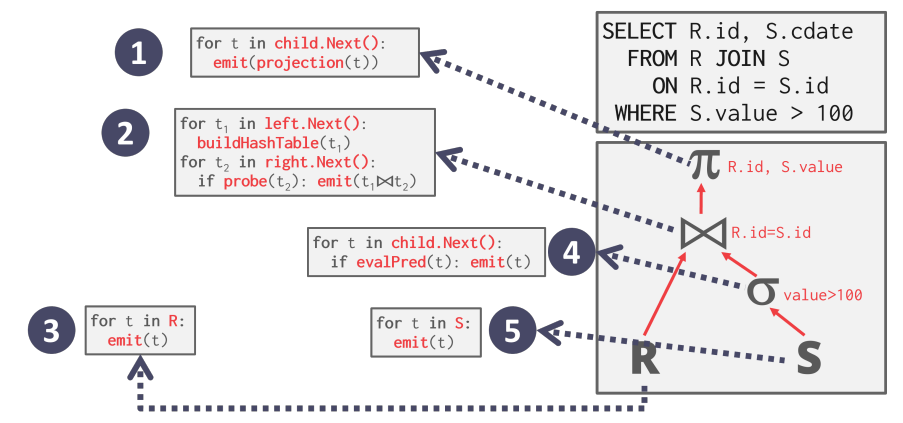
\includegraphics[width=0.7\linewidth]{screenshot001}

در اینجا شبه‌کد برای توابع Next برای هر یک از عملگرها آورده شده است. این توابع Next به طور اساسی حلقه‌های for هستند که بر روی خروجی عملگر فرزند خود تکرار می‌شوند. به عنوان مثال،ریشه Next را بر روی فرزند خود، عملگر join فراخوانی می‌کند. پس از پردازش همه ردیف‌ها، یک پوینتر null (یا پوینتر دیگری) ارسال می‌شود که به گره‌های والد اطلاع می‌دهد که به مرحله بعد بروند.




\pagebreak
\subsection{مدل Materialization‌}

مدل ماده‌سازی یک تخصصی از مدل تکرارگر است که در آن هر عملگر ورودی خود را به طور کامل پردازش کرده و سپس خروجی خود را به طور کامل منتشر می‌کند. به جای داشتن یک تابع Next که یک تاپل را برمی‌گرداند، هر عملگر همه تاپل‌های خود را هر بار که فراخوانی می‌شود، برمی‌گرداند. برای جلوگیری از اسکن تاپل‌های بیش از حد، DBMS می‌تواند اطلاعاتی درباره تعداد تاپل‌های مورد نیاز به عملگرهای بعدی منتقل کند. خروجی می‌تواند یا یک تاپل کامل (NSM) یا یک زیرمجموعه‌ای از ستون‌ها (DSM) باشد.

هر عملگر برنامه پرس‌وجو یک تابع Output را پیاده‌سازی می‌کند که:
\begin{enumerate}
	\item عملگر تمامی ردیف‌ها از فرزندان خود را یکجا پردازش می‌کند.
	
	\item نتیجه بازگشتی از این تابع تمامی ردیف‌هایی است که عملگر هرگز ارسال خواهد کرد. زمانی که عملگر اجرای خود را به پایان می‌رساند، DBMS هرگز نیازی ندارد که برای بازیابی داده‌های بیشتر به آن بازگردد.
\end{enumerate}

این رویکرد برای بارهای کاری OLTP بهتر است زیرا پرس‌وجوها معمولاً تنها به تعداد کمی از ردیف‌ها در هر زمان دسترسی دارند. بنابراین، فراخوانی‌های کمتری برای بازیابی ردیف‌ها وجود دارد. مدل Materialization برای پرس‌وجوهای OLAP با نتایج میانی بزرگ مناسب نیست زیرا ممکن است DBMS نیاز داشته باشد که آن نتایج را بین عملگرها به دیسک منتقل کند.

\qquad\qquad\qquad	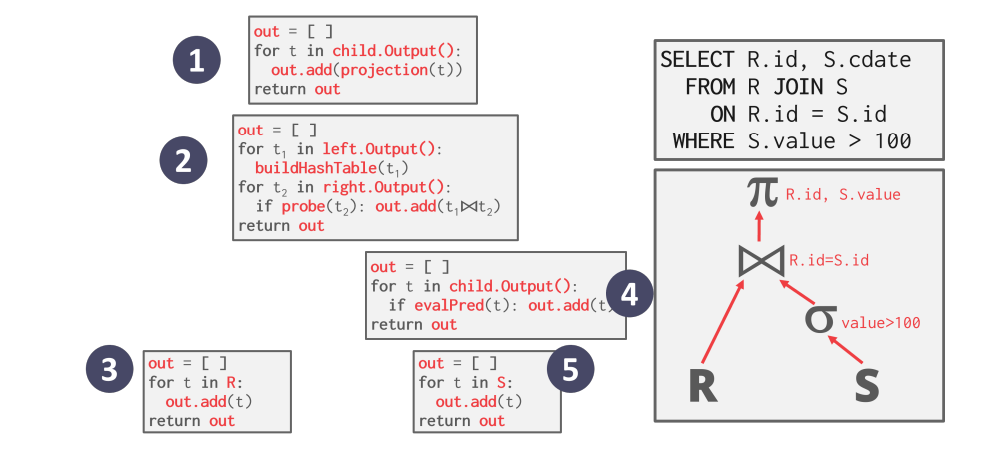
\includegraphics[width=0.7\linewidth]{screenshot002}

در مدل Materialization ، اجرای پرس‌وجو از گره ریشه شروع می‌شود و تابع Output فرزند فراخوانی می‌شود که عملگرهای زیرین را فراخوانی می‌کند و تمامی ردیف‌ها را به سمت بالا باز می‌گرداند. در شکل فوق شبه‌کد برای چگونگی اجرای این فرآیند برای هر عملگر آمده است.

\pagebreak

\subsection{مدل Vectorization}
مانند مدل iterator ، هر عملگر در مدل برداری یک تابع Next را پیاده‌سازی می‌کند. با این حال، هر عملگر یک دسته بردار از داده‌ها را به جای یک تاپل منتشر می‌کند. پیاده‌سازی حلقه داخلی عملگر برای پردازش دسته‌های داده به جای یک مورد در هر زمان بهینه شده است. اندازه دسته می‌تواند بر اساس سخت‌افزار یا ویژگی‌های کوئری متفاوت باشد.

\qquad\qquad\qquad	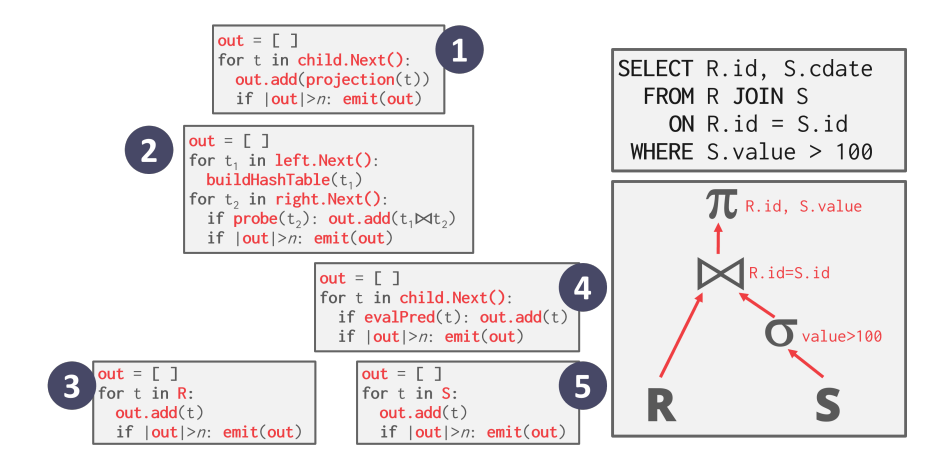
\includegraphics[width=0.7\linewidth]{screenshot003}

مدل بردارسازی بسیار شبیه به مدل Iterator است، به جز اینکه در هر عملگر، یک بافر خروجی با اندازه انتشار مورد نظر مقایسه می‌شود. اگر بافر بزرگتر باشد، یک دسته از ردیف‌ها به بالا ارسال می‌شود. این مدل با پردازش دسته‌ای از ردیف‌ها به جای پردازش تک‌تک ردیف‌ها در هر زمان، بهره‌وری بیشتری را به دست می‌آورد.

مدل بردارسازی به دلیل اینکه تعداد فراخوانی‌های تابع Next کمتر است، برای پرس‌وجوهای OLAP که نیاز به اسکن تعداد زیادی از ردیف‌ها دارند ایده‌آل است. این مدل به عملگرها اجازه می‌دهد تا به راحتی از دستورالعمل‌های برداری (SIMD) برای پردازش دسته‌ای از ردیف‌ها استفاده کنند.

\subsection{جهت پردازش}
\begin{itemize}
	\item رویکرد 1: از بالا به پایین
	\begin{itemize}
		\item با ریشه شروع کنید و داده‌ها را از فرزندان به والدین ``کشیده'' کنید.
		\item تاپل‌ها همیشه با فراخوانی توابع منتقل می‌شوند.
	\end{itemize}
	\item رویکرد 2: از پایین به بالا
	\begin{itemize}
		\item با برگ شروع کنید و داده‌ها را از فرزندان به والدین ``هل'' دهید.
		\item این رویکرد امکان کنترل دقیق‌تر حافظه‌های کش و رجیسترها در خطوط لوله عملگرها را فراهم می‌کند.
	\end{itemize}
\end{itemize}

\pagebreak

\section{روش‌های دسترسی}
به این که DBMS چگونه داده‌های ذخیره شده در یک جدول دسترسی پیدا می‌کند، روش دسترسی میگویند.

به طور کلی دو روش برای مدل‌های دسترسی وجود دارد: داده‌ها یا از یک جدول خوانده می‌شوند یا با یک اسکن ترتیبی از یک شاخص.
\subsection{اسکن ترتیبی}
عملگر اسکن ترتیبی روی هر صفحه در جدول تکرار می‌کند و آن را از حافظه پنهان بافر بازیابی می‌کند. هنگامی که اسکن روی تمام تاپل‌های هر صفحه تکرار می‌کند، گزاره را ارزیابی می‌کند تا تصمیم بگیرد که آیا تاپل را به عملگر بعدی منتشر کند یا نه.


اسکن ترتیبی جدول تقریباً همیشه ناکارآمدترین روش برای اجرای یک پرس و جو توسط یک DBMS است.


تعدادی بهینه‌سازی وجود دارد که به افزایش سرعت اسکن‌های ترتیبی کمک می‌کنند:
\begin{itemize}
	\item پیش‌دریافت: صفحات بعدی را از قبل دریافت کنید تا DBMS مجبور نباشد هنگام دسترسی به هر صفحه بر روی I/O ذخیره‌سازی متوقف شود.
	
	\item دور زدن حافظه پنهان بافر: عملگر اسکن صفحات دریافتی از دیسک را در حافظه محلی خود ذخیره می‌کند تا از سیل ترتیبی جلوگیری کند.
	
	\item موازی‌سازی: اسکن را با استفاده از چندین نخ / فرآیند به صورت موازی اجرا کنید.
	
	\item ماده‌سازی دیرهنگام:
	DBSM های 
	از نوع DSM
	می‌توانند به تأخیر انداختن به هم دوختن توپل‌ها تا بخش‌های بالای طرح پرس و جو را انجام دهند. این اجازه می‌دهد تا هر عملگر حداقل اطلاعات مورد نیاز را به عملگر بعدی منتقل کند.
	
	\item خوشه‌بندی پشته: توپل‌ها با استفاده از یک شاخص خوشه‌بندی در صفحات پشته ذخیره می‌شوند.
	
	\item پرس و جوهای تقریبی: پرس و جوها را بر روی یک زیرمجموعه نمونه‌برداری شده از کل جدول اجرا کنید تا نتایج تقریبی تولید کنید. این به طور معمول برای محاسبه تجمیع‌ها در یک سناریو انجام می‌شود که اجازه خطای کم را می‌دهد تا یک پاسخ تقریباً دقیق تولید شود.
	
	\item نقشه‌بندی منطقه‌ای: پیش‌محاسبه تجمیع‌ها برای هر ویژگی توپل در یک صفحه. DBMS سپس می‌تواند با بررسی نقشه منطقه‌ای خود ابتدا تصمیم بگیرد که آیا نیاز به دسترسی به یک صفحه دارد یا نه.
\end{itemize}

\qquad\qquad\qquad	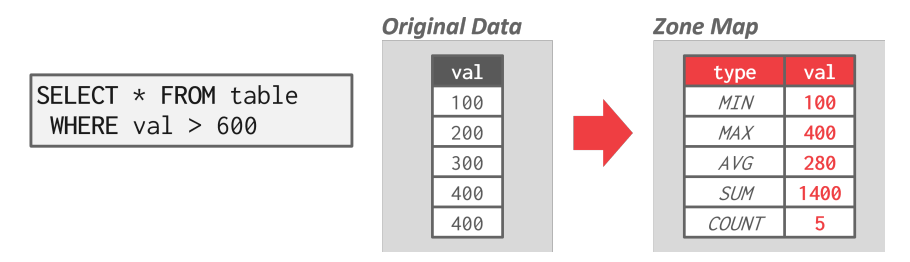
\includegraphics[width=0.7\linewidth]{screenshot004}

در مثال بالا، کوئری Select از Zone-Map متوجه می‌شود که حداکثر مقدار در داده‌های اصلی تنها ۴۰۰ است. 
سپس، به جای آن که مجبور باشد هر زوج مرتب در صفحه را بررسی کند، پرس و جو می‌تواند از دسترسی به صفحه به‌طور کامل اجتناب کند زیرا هیچ یک از مقادیر بزرگتر از ۶۰۰ نخواهند بود.



\subsection{اسکن شاخص}
در یک اسکن شاخص، DBMS یک شاخص را انتخاب می‌کند تا توپل‌هایی که یک پرس و جو نیاز دارد را پیدا کند.

\qquad\qquad\qquad	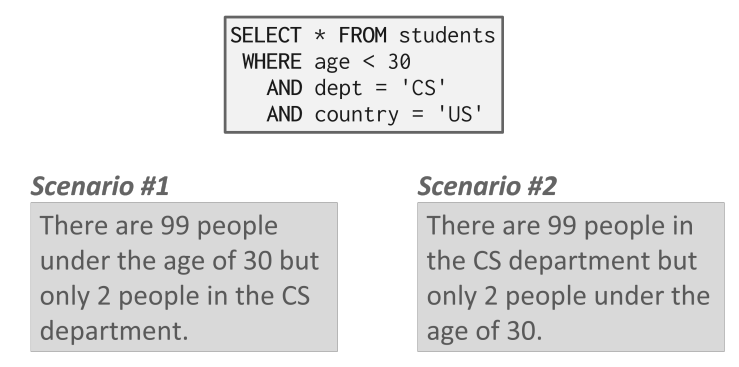
\includegraphics[width=0.7\linewidth]{screenshot005}

جدولی با ۱۰۰ زوج‌مرتب و دو ایندکس را در نظر بگیرید: سن و دپارتمان. 
در سناریوی اول، بهتر است از ایندکس دپارتمان در اسکن استفاده شود زیرا فقط دو زوج‌مرتب برای مطابقت دارد. 
انتخاب ایندکس سن خیلی بهتر از یک اسکن ترتیبی ساده نخواهد بود. 
در سناریوی دوم، ایندکس سن اسکن‌های غیرضروری بیشتری را حذف می‌کند و انتخاب بهینه است.


انتخاب شاخص توسط DBMS شامل عوامل بسیاری است:
\begin{itemize}
	\item چه ویژگی‌هایی در شاخص وجود دارند.
	\item چه ویژگی‌هایی پرس و جو را اشاره می‌کند.
	\item دامنه‌های مقداری ویژگی.
	\item ترکیب گزاره.
	\item اینکه آیا شاخص دارای کلیدهای یکتا یا غیر یکتا است.
\end{itemize}
DBMS
های پیشرفته‌تر از اسکن‌های چند شاخصی پشتیبانی می‌کنند. هنگام استفاده از چندین شاخص برای یک پرس و جو، DBMS مجموعه‌های آیدی های رکوردها را با استفاده از هر شاخص مطابقت داده شده محاسبه می‌کند، این مجموعه‌ها را بر اساس گزاره‌های پرس و جو ترکیب می‌کند، و رکوردها را بازیابی کرده و هر گزاره باقی‌مانده را اعمال می‌کند. DBMS می‌تواند از بیت‌مپ‌ها، جداول هش، یا فیلترهای بلوم برای محاسبه آیدی رکوردها از طریق تقاطع مجموعه‌ها استفاده کند.
\pagebreak

\section{کوئری‌های تعدیلی}
عملگرهایی که پایگاه داده را تغییر می‌دهند مسئول بررسی محدودیت‌ها و به‌روزرسانی شاخص‌ها هستند. 

برای UPDATE/DELETE ، عملگرهای فرزند شناسه‌های رکورد را برای تاپل‌های هدف منتقل می‌کنند و باید تاپل‌های قبلاً دیده شده را ردیابی کنند. دو انتخاب برای نحوه مدیریت عملگرهای INSERT وجود دارد:
\begin{itemize}
	\item انتخاب 1: تاپل‌ها را داخل عملگر ماده‌سازی کنید.
	\item انتخاب 2: عملگر هر تاپل انتقال یافته از عملگرهای فرزند را وارد می‌کند.
\end{itemize}


\qquad\qquad\qquad	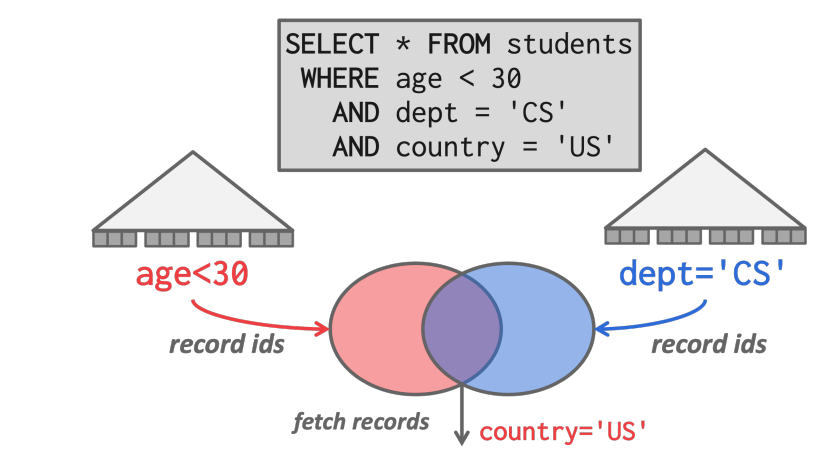
\includegraphics[width=0.7\linewidth]{screenshot006}

همان جدول در شکل قبل را در نظر بگیرید. با پشتیبانی از اسکن چند ایندکسی، ابتدا مجموعه‌های آیدی رکوردها که شرایط برای سن و دپارتمان را برآورده می‌کنند، به ترتیب با استفاده از ایندکس‌های مربوطه محاسبه می‌کنیم. سپس اشتراک دو مجموعه را محاسبه می‌کنیم، رکوردهای مربوطه را واکشی کرده و شرط باقی‌مانده \texttt{country='US'} را اعمال می‌کنیم.



\subsection{مشکل هالووین}
مشکل هالووین یک تناقض است که در آن یک عملیات به‌روزرسانی مکان فیزیکی یک تاپل را تغییر می‌دهد و باعث می‌شود یک عملگر اسکن چندین بار به تاپل مراجعه کند. این می‌تواند در جداول خوشه‌بندی شده یا اسکن‌های شاخص رخ دهد. این پدیده توسط محققان IBM در روز هالووین در سال 1976 هنگام ساخت System R کشف شد. راه حل این مشکل این است که شناسه‌های رکورد اصلاح شده را برای هر کوئری پیگیری شود.

\pagebreak

\section{ارزیابی عبارات}

DBMS
ها یک شرط WHERE را به عنوان یک درخت عبارت نمایش می‌دهد. گره‌ها در این درخت نوع‌های مختلف عبارت را نمایندگی می‌کنند.

\qquad\qquad\qquad	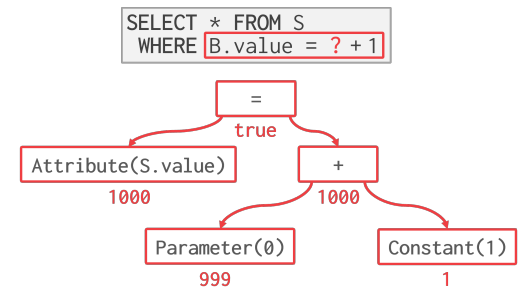
\includegraphics[width=0.7\linewidth]{screenshot007}


برخی از نمونه‌های نوع عبارات که می‌توانند در گره‌های درخت ذخیره شوند:
\begin{itemize}
	\item مقایسه‌ها (=, <, >, !=)
	\item And , Or
	\item عملگرهای حسابی (+, -, *, /, \%)
	\item مقادیر ثابت و پارامتر
	\item مراجع صفت تاپل
\end{itemize}

برای ارزیابی یک درخت عبارت در زمان اجرا، سیستم مدیریت پایگاه داده (DBMS) یک نگهدارنده زمینه را که حاوی فرا داده برای اجرا است، مانند زوج‌مرتب فعلی، پارامترها، و طرحواره جدول، نگهداری می‌کند. سپس DBMS درخت را پیمایش می‌کند تا عملگرهای آن را ارزیابی کرده و نتیجه‌ای تولید کند.

ارزیابی شرایط با این روش کند است زیرا DBMS باید کل درخت را پیمایش کرده و عمل صحیح را برای هر عملگر تعیین کند. رویکرد بهتر این است که عبارت را مستقیماً ارزیابی کنیم. بر اساس مدل هزینه داخلی، DBMS تعیین می‌کند که آیا تولید کد برای تسریع یک پرس‌وجو اتخاذ خواهد شد یا خیر.

\pagebreak
\section{برنامه‌ریز}

مدل‌های پردازش پرس‌وجوی بالا توصیف روشنی از جریان داده ارائه می‌دهند، در حالی که جریان کنترل نسبتاً ضمنی است. زمان‌بند جداسازی روشنی بین جریان داده و جریان کنترل دارد. این روش در حالت دسته‌ای، به‌ویژه مدل بُرداری، به خوبی کار می‌کند. زمان‌بند دستورات کاری را ایجاد می‌کند و به جای فراخوانی درخت عملگر از بالا به پایین، درخت را پیمایش کرده و کارهای زمان‌بندی را در صف زمان‌بندی قرار می‌دهد. سپس رشته‌های کاری درخواست‌ها را از صف واکشی کرده و آنها را اجرا می‌کنند.


\qquad\qquad\qquad	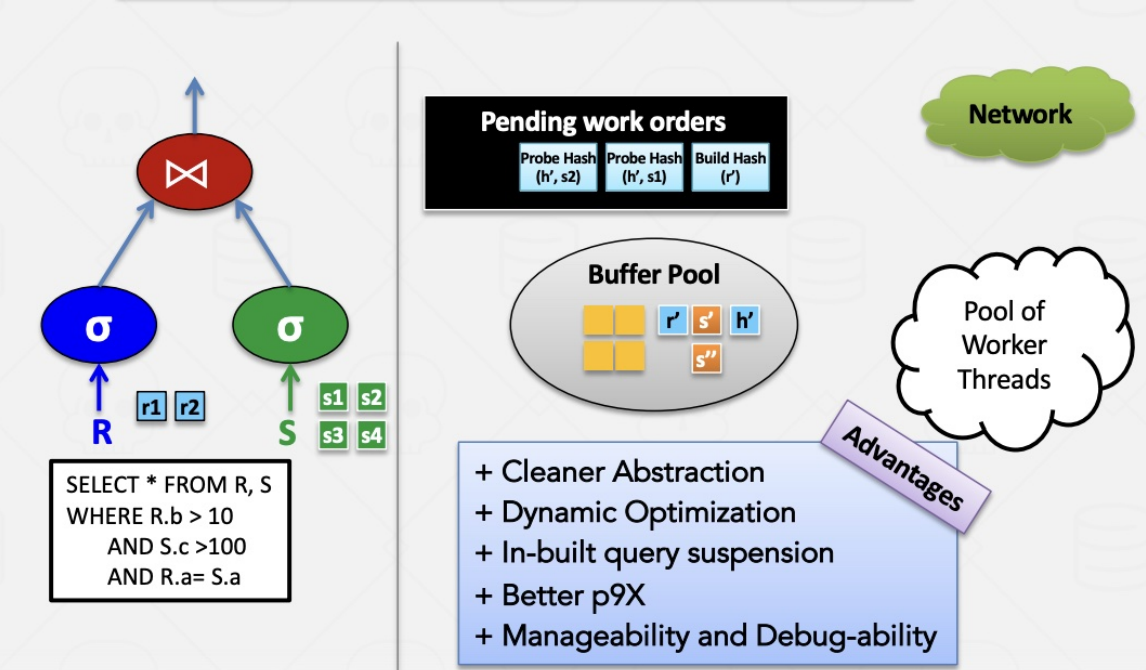
\includegraphics[width=0.7\linewidth]{screenshot008}

در شکل فوق مقایسه مدل پردازش پرس‌وجوی زمان‌بند و مدل پردازش پرس‌وجوی سنتی نشان داده شده است.

به طور کلی، این مدل دارای انتزاع تمیزتر، بهینه‌سازی پویا، تعلیق پرس‌وجوی داخلی، عملکرد بهتر و قابلیت مدیریت و اشکال‌زدایی بهتر است.










